% mainfile: ../../main.tex
\chapter{Conclusion \& outlook}\label{ch:setup:conclusion}
\AutoLettrine{In} \thispart I analyzed various aspects of the Millikelvin confocal microscope introduced in \citerr{Descamps2021}{Descamps2024}.
The setup offers the ability to conduct optical measurements of samples at Millikelvin temperatures while at the same time having access to state-of-the-art electrical wiring for sensitive quantum transport measurements such as those performed for semiconductor spin qubit experiments.
I first covered the refrigeration aspect of the setup in \cref{ch:setup:cooling}.
Housed in a commercial dry \gls{dr}, the modifications made for free-space optical access introduce additional heat loads and thus impact the available cooling power budget.
Specifically, I quantified the heat loads introduced by the motion stages' resistive position readout and irradiation of the sample with the laser, as well as the base temperature reached for different configurations of \gls{ar}-coated windows installed inside the cryostat.
With the optimal configuration of windows, I found the system to reach a base temperature below \qty{10}{\milli\kelvin} for readout voltages below \qty{100}{\milli\volt} and laser powers below \qty{10}{\micro\watt}.
To assess the impact on electrical performance, I measured the electron temperature in a \GaAsAlGaAs \acrlong{qd} in transport using Coulomb blockade thermometry.
I tuned a device designed for spin-qubit operation into a single \acrlong{qd} in the few-electron regime and measured the width of a conductance resonance in the sequential tunneling regime in direct transport, obtaining $T = \qty{75}{\milli\kelvin}$ comparable with state-of-the-art systems.

During these experiments, the objective was not focused onto the sample while the entrance window on top of the cryostat was not covered, allowing ambient light to enter.
As several studies have found, the electrical characteristics of \glspl{2deg} in \GaAsAlGaAs heterostructures, in particular \ch{Si}-doped ones, are highly sensitive to illumination, resulting in long-time transient effects and instabilities \cite{Fujita2021,Shetty2022,Wang2023,Reznikov2024}.
It would hence be interesting to study the behavior of electron temperature in relation to (wavelength-dependent) illumination, an experiment the setup described in \thispart is uniquely suited for.

In \cref{ch:setup:optics}, I then discussed the optical characteristics of the setup, in particular the microscope and its components.
I laid out the rationale behind choosing the lenses for collimating the Gaussian beam launched from the \gls{smf}, focusing it onto the sample, collecting the emitted radiation, and focusing that into another \gls{smf}.
Having chosen the lenses, I analyzed the efficiency of light emitted from a point dipole located inside a dielectric slab being coupled into the \gls{smf}.
From the analysis, it became clear that the precise spatial distribution of the electric field is non-trivial and warrants further attention.
A more detailed numerical simulation could serve to pinpoint areas of improvement besides fairly obvious solutions such as mirrors below the sample or mode-engineering like the approach pursued in \citer{Wu2024}.
On the other hand, measuring the field profile experimentally using a \gls{ccd} inserted into the optical path right before the detection fiber would allow better matching between theoretically expected and experimentally observed efficiencies.

\begin{marginfigure}[*-16]
    \begin{tikzpicture}[
    scale=2,%
    font=\footnotesize,%
    thick,%
    symmetryaxis/.style = {RWTHblack50,thin,dash dot},%
    lens/.style = {thick,<->},%
    optics/.style = {thick,black},%
    window/.style = {RWTHblue75,fill=RWTHblue25,text=black,opacity=0.75},%
    cryostat/.style = {RWTHblack75,thin,text=black},%
    midarrow1/.style = {postaction=decorate, decoration={markings,mark=at position 0.2 with \arrow{stealth}}},%
    midarrow2/.style = {postaction=decorate, decoration={markings,mark=at position 0.8 with \arrow{stealth}}},%
    midarrow/.style = {midarrow1, midarrow2},%
]    % requires libraries angle,calc,decorations.markings

    \ifdefined\ca
    \else
        \newlength\ca
    \fi
    \ifdefined\f
    \else
        \newlength\f
    \fi
    \ifdefined\dx
    \else
        \newlength\dx
    \fi
    \setlength\ca{0.25cm}
    \setlength\f{0.4cm}
    \setlength\dx{0.25cm}

    \coordinate (origin) at (0, 0);
    \coordinate (bs1) at (0, 0);
    \coordinate (mirror) at (0, -1.2);
    \coordinate (objective) at ($(mirror) + (0.6, 0)$);

    \coordinate (analyzer) at ($(bs1) + (0, 0.6)$);
    \coordinate (detection-ocular) at ($(analyzer) + (0, 1*\dx)$);

    \coordinate (polarizer) at ($(bs1) + (0.6, 0)$);
    \coordinate (excitation-ocular) at ($(polarizer) + (1*\dx, 0)$);

    \coordinate (source) at ($(objective) + (\f, 0)$);
    \coordinate (detection-fiber) at ($(detection-ocular) + (0, \f)$);
    \coordinate (excitation-fiber) at ($(excitation-ocular) + (\f, 0)$);

    % Symmetry axes
    \draw[symmetryaxis]
        ($(bs1) - (\ca*2,0)$)
        -- ($(excitation-fiber) + (\f/4,0)$)
    ;
    \draw[symmetryaxis]
        ($(mirror) - (0, \f/4)$)
        -- ($(detection-fiber) + (0, \f/4)$)
    ;
    \draw[symmetryaxis]
        ($(mirror) - (\f/4, 0)$)
        -- ($(source) + (\f/4, 0)$)
    ;

    % Beamsplitters
    \draw
    ($(bs1) - (1.5*\ca, 1.5*\ca)$) node[below left,xshift=2.1mm] {\acrshort{bs}1}
        -- ++($(3*\ca, 3*\ca)$)
    ;

    % Mirror
    \draw
        ($(mirror) + (-1.5*\ca, 1.5*\ca)$) node[above left,xshift=2.1mm] {M}
        -- ++($(3*\ca, -3*\ca)$)
    ;

    % Lenses
    \draw[lens]
        ($(objective) + (0, 1.5\ca)$)
        -- ++($(0, -3*\ca)$) node[below] {O}
    ;
    \draw[lens]
        ($(detection-ocular) - (1.5\ca, 0)$)
        -- ++($(3*\ca, 0)$) node[right] {D}
    ;
    \draw[lens]
        ($(excitation-ocular) + (0, 1.5\ca)$)
        -- ++($(0, -3*\ca)$) node[below] {E}
    ;

    % Optical elements
    \draw[optics]
        ($(polarizer) + (0, 1.5*\ca)$)
        -- ++($(0, -3*\ca)$) node[below] {P}
    ;
    \draw[optics]
        ($(analyzer) - (1.5*\ca, 0)$)
        -- ++($(3*\ca, 0)$) node[right] {A}
    ;

    % Excitation beam
    \draw[midarrow,RWTHred100]
        (excitation-fiber)
        -- ++($(-\f, -\ca)$)
        -- ($(bs1) - (\ca, \ca)$)
        -- ($(mirror) + (-\ca, \ca)$)
        -- ($(objective) + (0, \ca)$)
        -- (source)
    ;
    % Transmission
    \draw[midarrow2,RWTHred100]
        ($(bs1) - (\ca, \ca)$)
        -- ++($(-\ca, 0)$)
    ;
    % Detection beam
    \draw[midarrow,RWTHbordeaux100]
        (source)
        -- ++($(-\f, -\ca)$)
        -- ($(mirror) + (\ca, -\ca)$)
        -- ($(\ca, 0) + (detection-ocular)$)
        -- ++($(-\ca, \f)$)
    ;

\end{tikzpicture}

    \caption[\imgsource{img/tikz/setup/optical_path_reduced.tex}]{
        Reduced sketch of the optical path (\cf \cref{fig:setup:optics:optical_path}) including the cold mirror (M).
        The excitation laser experiences three reflections, twice at M and once at \acrshort{bs}1.
        The light emitted from the sample experiences a single reflection at M.
    }
    \label{fig:setup:conclusion:optical_path_reduced}
\end{marginfigure}

A crucial point might turn out to be the mirror in front of the objective lens.
As shown by \citet{Benelajla2021}, reflections of polarized non-plane-wave beams induce a modal transform into modes with nodes at the center that are spatially filtered by the \gls{smf} in a confocal geometry.
While beneficial for cross-polarization extinction (\cf \cref{subsec:setup:optics:coupling:rejection}), the same effect could lead to radiation emitted from the sample not coupling into the detection fiber if it is co-polarized with the excitation beam.\sidenote{
    Of course, the cross-polarization of analyzer and polarizer will suppress emitted radiation co-polarized with the excitation in any case.
    The excitation with linear polarization was chosen to coherently address exciton states in a Voigt configuration.
    If excitation with circularly polarized light is desired, the \quarterwave plate can be moved from the excitation arm to below \gls{bs}1 similar to \citer{Kuhlmann2013}.
    I tested this configuration but found the excitation rejection to be poor and reverted to the original configuration.
}
\Cref{fig:setup:conclusion:optical_path_reduced} shows a reduced sketch of the optical path.
Light emitted from the sample is reflected off the mirror (M) and passes through the \acrlong{bs} \acrshort{bs}1 and the analyzer (A) before being focused into the detection fiber by the ocular lens (D).
This situation is equivalent to that described by \citet{Benelajla2021} if the emitted light is cross-polarized with respect to A and has a Gaussian mode profile.
As I showed in \cref{subsec:setup:optics:coupling:efficiency}, the mode overlap between the dipole radiation after collimation and a Gaussian \TEM{00} mode is quite large at \qty{83}{\percent}, implying that the effects investigated in \citer{Benelajla2021} for Gaussian beams will also apply to some extent to the dipole radiation considered here.

For the excitation rejection, the cold mirror potentially adds another issue.
As shown by \citet{Steindl2023}, the giant cross-polarization extinction mechanism in a confocal geometry discovered by \citet{Benelajla2021} is reduced in efficacy when additional reflections are introduced into the optical path.\sidenote{
    A halfwave plate inserted into the path was also found to reduce the rejection ratio, suggesting that the \halfwave and \quarterwave plates might also impact performance.
    On the other hand, \citet{Kuhlmann2013} found the \quarterwave plate to be crucial for compensating ellipticities introduced by the setup.
}
Our situation is again slightly different to the one studied there, however, as the cold mirror is mounted perpendicular to the \gls{bs}\sidenote{
    That is, while $x$ lies in the plane of the \gls{bs}, $y$ lies in the plane of the cold mirror if we use the coordinate system of \cref{fig:setup:vibrations:knife_edge:sketch} where $x$ is the out-of-plane sample coordinate and $z$ is along gravity.
}
and hence the effects on $s$- and $p$-polarizations upon reflection mix.
A detailed analysis of the spatial mode profile would thus help elucidate the extent to which these effects matter in our experiments.

Lastly, in \cref{ch:setup:vibrations}, I addressed the impact of vibrations, induced chiefly by the \gls{ptr}, on the microscope performance.
After outlining the basic principles of vibration isolation, I described the suspension scheme based on passive air springs which I installed in the setup to mitigate the vibration noise coupled into system by the \gls{ptr}.
I then performed measurements of the displacement noise \gls{psd} using two different methods.
First, using a piezoelectric accelerometer that is directly sensitive to absolute displacements through the local acceleration experienced by the sensor, I found that during operation of the cryostat the vibrations should be considered too large for operation of the microscope, obtaining $\flatfrac{1}{3}$ octave band \gls{rms} velocities well into the tenths of \unit{\milli\meter\per\second} range.
However, I argued that the absolute value of displacement noise at the sample position is less indicative of the microscope performance than the relative displacement noise between sample and detection fiber, \ie, the vibrations along the optical path.
To quantify these, I introduced an optical \emph{in-situ} method of measuring lateral displacement using a knife-edge measurement on a reflectance step on a sample.
This technique can be employed without additional modifications or instruments besides those already present in the optical setup.
It is based on the fact that the finite spot size of the Gaussian laser beam incident on a step-like reflectance profile such as that produced by a lithographic \ch{Au} gate on a crystalline surface results in a linear slope in reflected intensity over the width of the laser spot.
This allows measuring the reflected intensity as function of time and subsequently converting the intensity to a displacement along the gradient using a previous calibration akin to the charge sensing technique in \glspl{gdqd}, following which the tools laid out in \cref{part:speck} can be used to obtain the noise \gls{psd}.
Using this technique, I showed that the relative displacement noise is orders of magnitude smaller than the absolute, placing the octave band \gls{rms} velocities well below the targeted levels categorized by the \acrlongpl{vc}.
I furthermore analyzed the sensitivity of the technique, showing that the noise floor is dominated by photon shot noise, and laid out routes for enhancing the \gls{snr}.

\Cref{fig:setup:conclusion:vibrations} summarizes the performance of the vibration damping for enabled \gls{ptr} and the two different vibration spectroscopy techniques.
The upper panel shows the relative (instantaneous) displacement noise power for activated suspension referenced to that for deactivated suspension (\cf \cref{subsec:speck:software:features:serial}) on a logarithmic scale.
The suspension appears to have a greater effect overall for the absolute level measured with the accelerometer.
However, looks can be deceiving as evidenced by the lower panel, which shows the integrated data,
\begin{equation}
    \mr{Integrated} \equiv 10\log_{10}\left(\frac{\rms_{S}^2(f)}{\rms_{\mr{ref}}^2(f)}\right),
\end{equation}
also on a logarithmic scale (\cf \cref{eq:setup:vibrations:rms}).
Clearly, above \qty{10}{\hertz} the suspension improves the overall noise power as measured by the optical method, whereas the absolute level measured with the accelerometer does not recover from the penalty taken between \qtylist{1;10}{\hertz} where oscillations are amplified by the air springs.

\begin{marginfigure}[*-15]
    \centering
    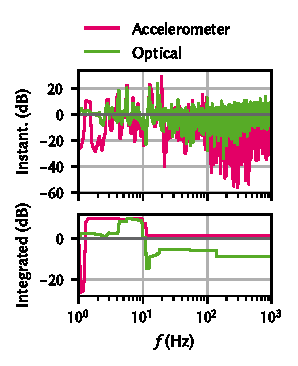
\includegraphics{img/pdf/setup/spect_dB}
    \caption[\imgsource{img/py/setup/vibration_spectroscopy.py}]{
        Relative displacement noise power of the setup with air spring suspension activated referenced to suspension deactivated.
        Lower panel shows the fractional integrated data.
    }
    \label{fig:setup:conclusion:vibrations}
\end{marginfigure}

The microscope characterized in \thispart has potential applications beyond the field of quantum technology.
Low-temperature effects such as superconductivity and other correlated electronic phases could be studied optically~\cite{Hadfield2016,Arora2020,Zhang2023}.
Van der Waals heterostructures appear particularly promising as they allow to combine optically responsive direct-gap semiconductors with metallic materials whose electronic properties can be studied in transport, leading to hybridization and proximity effects due to the atomically close contact~\cite{Geim2013}.
Examples of this include stacks of graphene or \gls{blg} with \glspl{tmd} such as \ch{MoS2} or \ch{WSe2}~\cite{Popert2022,Masseroni2024,Xie2024,Seiler2025}.
The latter display giant exciton binding energies that are sensitive to the dielectric screening by their close environment, thus allowing to serve as optical sensors of electronic properties~\cite{Popert2022,Tebbe2023}.
Recent experiments in this direction undertaken in the setup by \citet{Tebbe2025} on \acrshort{blg}/\ch{WSe2} show promising first results on \gls{soi} proximity effects and magnetic phases in \gls{blg}~\cite{Icking2024}.

\paragraph{Acknowledgements}
Parts of the results presented in \thispart have been published in \citer{Descamps2024}.
Thomas Descamps and Feng Liu originally designed the setup together with Hendrik Bluhm and constructed it.
Julian Ritzmann and Arne Ludwig grew the wafer on which Matthias Künne fabricated the sample used to measure the electron temperature in \cref{sec:setup:cooling:etemp}.
The chip used to measure photon antibunching in \cref{sec:setup:optics:g2} was grown by Xuelin Jin.
Marcus Eßer kindly lent the accelerometer used in \cref{sec:setup:vibrations:accel}.